\subsubsection{Component Tests with the Rate Reward}

\label{sec:rate_ablation}

We test five changes: remove graph features, remove rule features,
remove the action mask, remove training call cost, or use a small count
penalty. Ten seeds and 250 episodes per setting train fifty new models.
The ten existing rate-DDQN checkpoints give the full-policy baseline.
Thirty further corruptions of the same base graph give 2,100 outcomes,
including the heuristic. We evaluate every fixed model.

Feature removal sets the chosen inputs to zero during training and testing.
Other inputs and the mask stay available. The no-mask setting chooses
from all eight actions during action selection and target updates.
Unavailable graph actions can leave the graph unchanged. Repeated
acquisition can incur call cost. The no-call-cost setting removes that
training reward term. Evaluation uses the shared rate reward.

\begin{table}[t]

\centering

\caption{Rate-reward component tests. Values average ten seed means, each from thirty shared scenarios. Calls count simulated acquisition units. API requests are zero.}

\label{tab:rate_ablation}

\scriptsize

\begin{tabular}{lrrrr}

\toprule

Setting & F1 & Restoration & Calls & Unavailable \\

\midrule

Rate DDQN & 0.9952 & 0.9377 & 4.45 & 0.00 \\

No graph features & 0.9941 & 0.8938 & 4.10 & 0.00 \\

No rule features & 0.9775 & 0.6682 & 7.39 & 0.00 \\

No action mask & 0.9702 & 0.5776 & 6.23 & 8.26 \\

No call penalty & 0.9854 & 0.7686 & 5.54 & 0.00 \\

Small count penalty & 0.9905 & 0.9214 & 4.89 & 0.00 \\

Acquire-then-deficit & 0.9991 & 0.9884 & 4.00 & 0.00 \\

\bottomrule

\end{tabular}

\end{table}

Removing the mask lowers F1 by 2.50 points
(95\% seed-bootstrap CI: $[-3.45,-1.62]$; Holm $p=0.0234$).
It gives 8.26 unavailable choices per episode. This is the one comparison
with adjusted $p<0.05$ among twelve F1 and restoration tests.
Removing rule features lowers mean F1 and raises acquisition cost;
its adjusted $p>0.05$. Every setting keeps all initially correct
reference facts. The heuristic reaches the highest mean F1, 99.91\%.

\paragraph{Testing penalty size.}

Twenty development rollouts sample allowed actions uniformly.
We set the count coefficient to total rate burden divided by total new
violations: $\alpha=0.000164493$. Calibration uses observed graph changes.
Small-count DDQN reaches 99.05\% F1; rate DDQN reaches 99.52\%.
The paired difference is $-0.47$ points
(CI: $[-1.73,0.46]$, Holm $p=1$). The interval includes zero at
the base graph size.

\begin{figure*}[t]

\centering

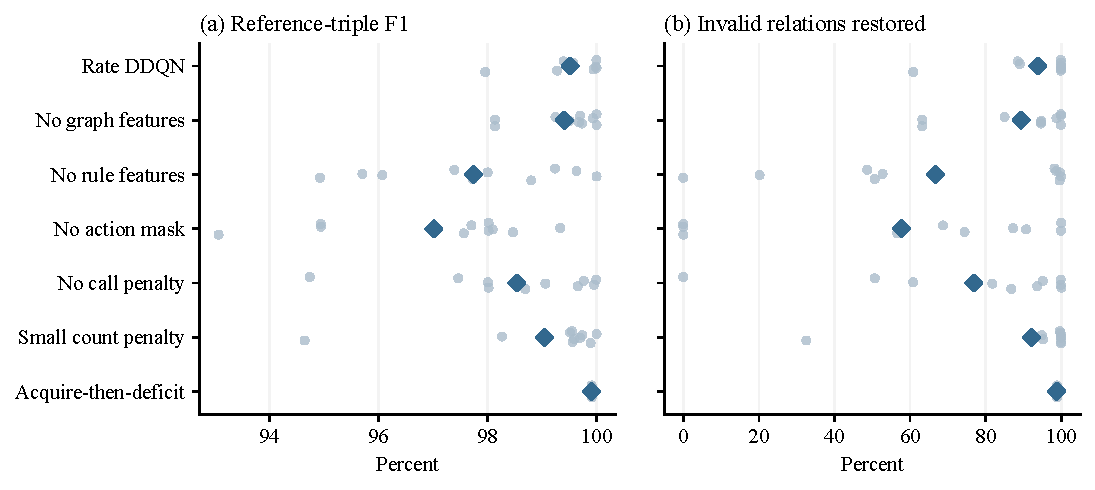
\includegraphics[width=0.93\textwidth]{figure/experiments/rate_ablation.pdf}

\caption{Rate-reward component tests and small-count control. Dots show ten training-seed means; diamonds show their average. Each mean uses thirty shared scenarios. The heuristic uses a fixed rule.}

\label{fig:rate_ablation}

\end{figure*}
